\chapter{Background} \label{ch:background}

This chapter provides an overview of the problem of portfolio optimisation in the financial domain, followed by a comprehensive explanation of the fundamentals of \acrfull{dl} and \acrfull{rl}, including the relevant algorithms in the field of \acrfull{drl}. In addition, it discusses the need for explainability in \acrfull{ml} and the main techniques used to achieve it: \acrfull{shap}, \acrfull{lime} and \Gls{featureimportance}. Finally, it presents the state of the art in portfolio optimisation using \acrshort{drl} and the recent advancements in explainability techniques in the field. 

\section{Portfolio Optimisation} \label{sec:portfoliooptimisation}

\Gls{portfoliooptimisation} is the process of selecting optimal weights for a portfolio of assets in order to maximise expected returns for a given level of risk, or conversely, to minimise risk for a given level of expected returns \cite{Sato2019}. In mathematical terms, the problem requires finding a solution to the specified objective function, which is typically a function of the expected returns and the risk associated with the portfolio \cite{Bruce2014}. The task becomes further complicated if a time dimension is introduced, as the portfolio weights need to be adjusted over time to capture the changes in market conditions and asset prices \cite{Li2019}. 

\subsection{Modern Portfolio Theory}

There exist several traditional frameworks that formalise the problem of portfolio allocation. Markowitz's \acrfull{mpt} was proposed in 1952 \cite{Markowitz1952} and it provides a mathematical framework where investors choose optimal portfolios based on risk and return, by either minimising the risk given a specified return or, maximising the return given a specified risk \cite{kent}. The theory extends the concept of diversification by suggesting that owning financial assets of different kinds is less risky than owning assets of the same kind, due to the correlations between assets. 

The main assumptions in \acrshort{mpt} are:
\begin{itemize}
    \item investors are risk-averse, rational, and seek to maximise return for a given risk;
	\item returns are normally distributed;
	\item markets are frictionless, meaning there are no transaction costs; and
	\item assets are infinitely divisible.
\end{itemize}

Under these assumptions, portfolio risk and return can be modelled as an optimisation problem. Let $\mathbf{w} = \left(w_1, w_2, \dots, w_N\right)^T$ denote the portfolio weight vector, where each $w_i$ indicates the proportion of capital allocated to asset $i$, subject to the budget constraint:
\begin{equation}
    \sum_{i=1}^{N} w_i = 1 \quad \Leftrightarrow \quad \mathbf{w}^T \mathbf{1} = 1
\end{equation}
with $\mathbf{1} \in \mathbb{R}^N$ being a vector of ones, and subject to the non-negativity constraint, meaning that short-selling is not allowed:
\begin{equation}
    w_i \geq 0 \quad \forall i = 1, 2, \dots, N.
\end{equation}

Let $\boldsymbol{\mu} = \left(R_1, R_2, \dots, R_N\right)^T$ represent the vector of expected returns, and $\Sigma \in \mathbb{R}^{N \times N}$ the covariance matrix of asset returns. The expected return of the portfolio is then given by:
\begin{equation}
    R_p = \mathbf{w}^T \boldsymbol{\mu},
\end{equation}
and the portfolio risk is quantified by the variance of returns:
\begin{equation}
    \sigma_p^2 = \mathbf{w}^T \Sigma \mathbf{w}.
\end{equation}

This formulation provides the foundation for solving the mean-variance optimisation problem, by either:
\begin{itemize}
    \item minimising portfolio variance $\sigma_p^2$ subject to a target expected return $R_p$, or
    \item maximising expected return $R_p$ subject to a risk constraint $\sigma_p$.
\end{itemize}

The Markowitz mean-variance optimisation problem can be expressed as:
\begin{equation}
\begin{aligned}
    \min_{\mathbf{w}} \quad & \mathbf{w}^T \Sigma \mathbf{w} \\
    \text{subject to} \quad &
    \begin{cases}
        \mathbf{w}^T \boldsymbol{\mu} = R_p \\
        \mathbf{w}^T \mathbf{1} = 1 \\
        \mathbf{w} \geq 0
    \end{cases}
\end{aligned}
\end{equation}

Solving the mean-variance optimisation problem for varying levels of target return leads to a set of optimal portfolios that form the \gls{efficientfrontier}. It is typically visualised in a risk-return space, where the x-axis represents the risk (standard deviation) and the y-axis represents the expected return, as shown in Figure \ref{fig:efficient_frontier}. Portfolios below the curve are suboptimal, while those on the frontier represent the best achievable combinations of risk and return.

\begin{figure}[ht]
    \centering
    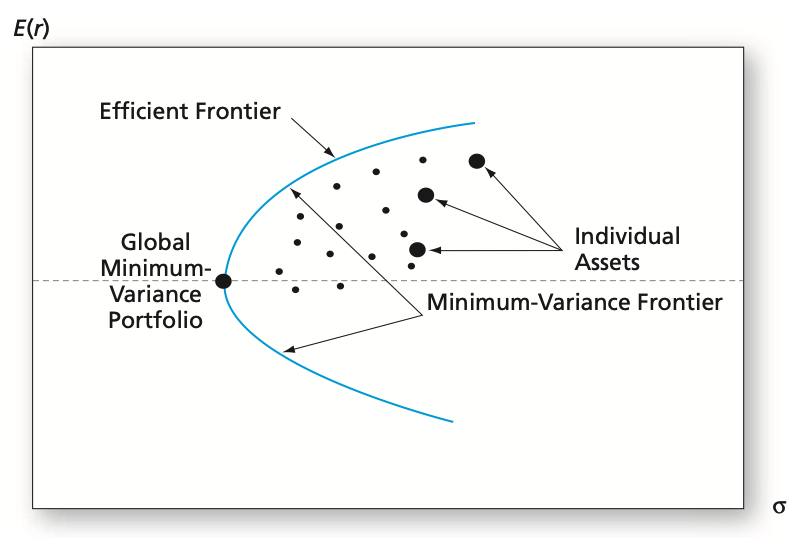
\includegraphics[width=0.8\textwidth]{figures/markowitz-efficient-frontier.png}
    \caption{Efficient Frontier in Risk-Return Space. \cite{Bodie2014}}
    \label{fig:efficient_frontier}
\end{figure}

Despite the simplicity in the formulation of \acrshort{mpt}, its assumptions do not reflect the behaviour of real markets. Moreover, modern markets are dynamic, non-stationary, and feature non-linear relationships, which have driven research into other approaches better suited to capture the complexities of modern financial markets. 
 
\section{Deep Reinforcement Learning} \label{sec:deepreinforcementlearning}

\acrlong{ml} is a branch of \acrfull{ai} that focuses on the use of data and algorithms to imitate the way humans learn, gradually improving their accuracy over time \cite{IBM2021}. There are three main tasks in \acrshort{ml} \cite{Francois-Lavet2018}:

\begin{itemize}
    \item \textbf{\Gls{supervisedlearning}}: Task of training a classification or regression model from labelled training data, where the model learns to map inputs to outputs based on examples.
    \item \textbf{\Gls{unsupervisedlearning}}: Task of drawing inferences from datasets consisting of unlabelled input data, where the model learns to identify patterns or structures in the data.
    \item \textbf{\acrlong{rl}}: Task of training an agent to sequentially make decisions by taking actions in an environment with the goal of maximising cumulative reward, using feedback from the environment to learn an optimal strategy.
\end{itemize}

\acrlong{dl} is a set of methods and techniques to solve such \acrshort{ml} tasks, specially in supervised and unsupervised learning tasks. \acrshort{dl} focuses on the use of \acrfull{dnn} \cite{Goodfellow2016}, which are characterised by a succession of layers of non-linear transformation that allow the model to learn a representation of the data with various levels of abstraction.

Therefore, \acrfull{drl} combines \acrfull{dl} and \acrfull{rl} to solve sequential decision-making problems with high-dimensionality in the environment representation. This approach has gained significant attention in recent years due to its success in various applications, including robotics \cite{Tang2024} and game playing \cite{Silver2016, Shao2019}.

\subsection{Reinforcement Learning} \label{sec:reinforcementlearning}

As mentioned, \acrshort{rl} is a type of \acrshort{ml} that solves the problem of sequential decision-making through continuous interaction with an environment. The agent learns to take actions given a representation of the environment's state with the goal of optimising a pre-defined notion of reward. The agent learns by successively adjusting its policy based on its observations and interactions with the environment. 

The \acrshort{rl} problem can be formalised as a discrete-time stochastic control process where an agent interacts with the environment. At each time step $t$, the agent observes the state of the environment $s_t \in \mathcal{S}$, takes an action $a_t \in \mathcal{A}$ to obtain a reward $r_t \in \mathbb{R}$ and transition to a new state $s_{t+1} \in \mathcal{S}$, where $\mathcal{S}$ is the state space and $\mathcal{A}$ is the action space \cite{Francois-Lavet2018}. The agent's interaction with the environment is visually represented in Figure \ref{fig:agent_environment_interaction}.

\begin{figure}[ht]
    \label{fig:agent_environment_interaction}
    \centering
    \begin{tikzpicture}[>=stealth]
    % Nodes
    \node[draw, rectangle, minimum width=2cm, minimum height=1cm] (agent) {Agent};
    \node[draw, rectangle, minimum width=2.8cm, minimum height=1cm, right=5cm of agent] (env) {Environment};

    % Coordinates for paths
    \coordinate (top1) at ($(env.north)+(0,1.5)$);
    \coordinate (top2) at ($(agent.north)+(0,1.5)$);

    \coordinate (bot1) at ($(env.south)+(0,-1.5)$);
    \coordinate (bot2) at ($(agent.south)+(0,-1.5)$);

    % Arrows
    \draw[->] (agent) -- node[above, midway] {Action $a_t$} (env);
    \draw[->] (env.north) -- (top1) -- node[above] {State $s_t$} (top2) -- (agent.north);
    \draw[->] (env.south) -- (bot1) -- node[below] {Reward $r_t$} (bot2) -- (agent.south);
\end{tikzpicture}
    \caption{Agent interaction with environment}
\end{figure}

A discrete time stochastic control process can be formalised as a \acrfull{mdp}, if it fulfils the Markov Property. 

\begin{definition}[Markov Property]
    A discrete time stochastic control process satisfies the Markov Property if:
    \begin{eqnarray}
        P(s_{t+1} | s_t, a_t) = P(s_{t+1} | s_t, a_t, s_{t-1}, a_{t-1}, \dots, s_0, a_0) \\  
        P(r_t | s_t, a_t) = P(r_t | s_t, a_t, s_{t-1}, a_{t-1}, \dots, s_0, a_0)
    \end{eqnarray}
    where $P(s_{t+1} | s_t, a_t)$ is the transition probability of moving to state $s_{t+1}$ given the current state $s_t$ and action $a_t$, and $P(r_t | s_t, a_t)$ is the reward function that defines the expected reward received at time $t$ given the current state and action.
\end{definition}

This implies that the state $s_{t+1}$ at a future time step $t+1$ only depends on the current state $s_t$ and action $a_t$. Similarly, the reward $r_t$ at time step $t$ only depends on the current state and action and not on the history of previous states and actions. Consequently, a \acrlong{mdp} \cite{Bellman1957} is a discrete time stochastic control process defined as:

\begin{definition}[Markov Decision Process]
    An \acrshort{mdp} is a tuple $\mathcal{M} = \left(\mathcal{S}, \mathcal{A}, T, R, \gamma\right)$, where:
    \begin{itemize}
        \item $\mathcal{S}$ is the state space: $s_t \in \mathcal{S}$,
        \item $\mathcal{A}$ is the action space: $a_t \in \mathcal{A}$,
        \item $T: \mathcal{S} \times \mathcal{A} \times \mathcal{S} \rightarrow [0, 1]$ is the transition function,
        \item $R: \mathcal{S} \times \mathcal{A} \times \mathcal{S} \rightarrow \mathcal{R}$ is the reward function, where $\mathcal{R} \in \left[0, R_{max}\right]$ is the set of all possible rewards bounded by $R_{max} \in \mathbb{R}^+$, and
        \item $\gamma \in [0, 1)$ is the discount factor.
    \end{itemize}
    
\end{definition}

At each time step, the probability of advancing to the next state $s_{t+1}$ is given by the transition function $T(s_t, a_t, s_{t+1})$ and the reward $r_t$ is given by the reward function $R(s_t, a_t, s_{t+1})$. This can be visualised in Figure \ref{fig:mdp}.

\begin{figure}[ht]
    \label{fig:mdp}
    \centering
    \begin{tikzpicture}[->, >=stealth, node distance=2cm, every node/.style={scale=0.9}]
    % State nodes
    \node[circle, draw, minimum size=1cm] (s0) {$s_0$};
    \node[circle, draw, minimum size=1cm, right=4cm of s0] (s1) {$s_1$};
    \node[circle, draw, minimum size=1cm, right=4cm of s1] (s2) {$s_2$};

    % Action nodes
    \node[circle, draw, minimum size=1cm, below=2cm of s0] (a0) {$a_0$};
    \node[circle, draw, minimum size=1cm, below=2cm of s1] (a1) {$a_1$};

    % Reward nodes
    \node[circle, draw, minimum size=1cm, right=2.5cm of a0] (r0) {$r_0$};
    \node[circle, draw, minimum size=1cm, right=2.5cm of a1] (r1) {$r_1$};

    % Arrows between states
    \draw[->] (s0) -- (s1) node[midway, above] {\begin{tabular}{c}
            Transition function \\
            $T(s_0, a_0, s_1)$
        \end{tabular}};
    \draw[->] (s1) -- (s2) node[midway, above] {\begin{tabular}{c}
            Transition function \\
            $T(s_1, a_1, s_2)$
        \end{tabular}};

    % Policy arrows 
    \draw[->] (s0) -- (a0) node[midway, left] {Policy};
    \draw[->] (s1) -- (a1) node[midway, left] {Policy};

    \draw[->] (a0) .. controls +(0,3.7) and +(0,3.7) .. node[midway, below, yshift=-20pt] {\begin{tabular}{c}
            Reward function \\
            $R(s_0, a_0, s_1)$
        \end{tabular}} (r0);

    \draw[->] (a1) .. controls +(0,3.7) and +(0,3.7) .. node[midway, below, yshift=-20pt] {\begin{tabular}{c}
            Reward function \\
            $R(s_1, a_1, s_2)$
        \end{tabular}} (r1);

    % Ellipsis
    \node at ($(s2)+(1.2cm,0)$) {\large $\cdots$};

\end{tikzpicture}
    \caption{Markov Decision Process with policy, transition, and reward functions}
\end{figure}

The agent's objective is to learn a policy $\pi: \mathcal{S} \rightarrow \mathcal{A}$ that maps states to actions, in order to maximise the expected cumulative reward over time. Policies can be categorised as:
\begin{itemize}
    \item deterministic: $\pi(s) : \mathcal{S} \to \mathcal{A}$, at a given state $s$, the policy specifies the only available action to take, or
    \item stochastic: $\pi(s, a) : \mathcal{S} \times \mathcal{A} \to [0, 1]$, at a given state $s$, the policy specifies the probability of taking action $a$.
\end{itemize}

\acrlong{mdp} are based on the idea that the current state is fully representative of the environment. However, in most real world scenarios, the agent does not have access to the complete state. In such cases, \acrfull{pomdp} can be used to model the uncertainty in the agent's observations and actions.

The goal of the agent is to maximise the cumulative long-term reward $G_t$, which is defined as the sum of discounted rewards over time:
\begin{equation}
    G_t = r_{t+1} + \gamma r_{t+2} + \gamma^2 r_{t+3} + \dots = r_{t+1} + \gamma G_{t+1}
\end{equation}
where $\gamma \in [0, 1)$ is the discount factor and is used to balance the importance between immediate and future rewards. If the discount factor is set to 0, the agent is myopic and only maximises the immediate reward; whereas, as $\gamma$ approaches $1$, the agent becomes more far-sighted and places greater importance on future rewards.

The expected cumulative reward is defined as the state value function $V^\pi(s): \mathcal{S} \to \mathbb{R}$, which is the expected return when starting from state $s$ and following policy $\pi$:
\begin{equation}
    V^\pi(s) = \mathbb{E}_\pi \left[G_t | s_t = s\right] 
\end{equation}
where $\mathbb{E}_\pi$ denotes the expectation over the policy $\pi$.

Similarly, the state-action value function $Q^\pi(s, a): \mathcal{S} \times \mathcal{A} \to \mathbb{R}$ is defined as the expected return when starting from state $s$, taking action $a$, and then following policy $\pi$:
\begin{equation}
    Q^\pi(s, a) = \mathbb{E}_\pi \left[G_t | s_t = s, a_t = a\right] 
\end{equation}

The state value function $V^\pi(s)$ and the state-action value function $Q^\pi(s, a)$ are related as follows:
\begin{equation}
    V^\pi(s) = \sum_{a \in \mathcal{A}} \pi(a | s) Q^\pi(s, a) = \mathbb{E}_\pi \left[Q^\pi(s, a) \mid s_t = s\right]
\end{equation}

Moreover, the advantage function $A^\pi(s, a)$ combines both the state value function $V^\pi(s)$ and the state-action value function $Q^\pi(s, a)$, and is defined as:
\begin{equation}
    A^\pi(s, a) = Q^\pi(s, a) - V^\pi(s)
\end{equation} 

A policy $\pi$ is said to be optimal if the policy's value function is the optimal value function of the \acrshort{mdp}, defined as: 
\begin{eqnarray}
    V^*(s) = \max_{\pi'} V^{\pi'}(s), \forall s \in \mathcal{S} \\ 
    Q^*(s, a) = \max_{\pi'} Q^{\pi'}(s, a), \forall s \in \mathcal{S}, a \in \mathcal{A}
\end{eqnarray}
The optimal policy $\pi^*$ is:
\begin{equation}
    \pi^*(s) = \arg \max_{a\in \mathcal{A}} Q^*(s, a)
\end{equation}

As a result, the optimal policy is the greedy policy that performs the optimal actions at each time step as determined by the optimal value functions. This framework enables the agent to determine optimal actions that maximise long-term returns by evaluating immediate information, without requiring knowledge of the values of future states and actions.

The \Gls{bellmanequations} \cite{Bellman1957book} provide a recursive relation between the value functions in terms of the future state/action values. There are four main Bellman equations, classified in two groups: the Bellman expectation equations and the Bellman optimality equations. The Bellman expectation equations are defined as follows:
\begin{eqnarray}
    V^\pi(s) = \sum_{a \in \mathcal{A}} \pi\left(a \mid s\right) \sum_{s'\in \mathcal{S}} T\left(s, a, s'\right) \left[R\left(s,a\right) + \gamma V^\pi(s')\right] \\ 
    Q^\pi(s, a) = \sum_{s'\in \mathcal{S}} T\left(s, a, s'\right) \left[R\left(s,a\right) + \gamma \sum_{a' \in \mathcal{A}} \pi\left(a' \mid s'\right) Q^\pi(s', a')\right]
\end{eqnarray}

and the Bellman optimality equations are defined as:
\begin{eqnarray}
    V^*(s) = \max_{a \in \mathcal{A}} \sum_{s'\in \mathcal{S}} T\left(s, a, s'\right) \left[R\left(s,a\right) + \gamma V^*(s')\right] \\
    Q^*(s, a) = \sum_{s'\in \mathcal{S}} T\left(s, a, s'\right) \left[R\left(s,a\right) + \gamma \max_{a' \in \mathcal{A}} Q^*(s', a')\right]
\end{eqnarray}

Although explicitly solving the Bellman equations would lead to the optimal policy, it is often intractable due to the size of the state and action spaces. Therefore, in \acrshort{rl} algorithms, the goal is to learn an approximation of the optimal value functions, which can be used to derive the optimal policy. Another problem that arises is that of balancing exploration and exploitation \cite{Thrun1992}. Theoretically, following the greedy action yields the optimal policy, but this is only true if all the action values are known. In practice, the agent at each time step and given state chooses either an action whose value is higher, thus exploiting its current knowledge, or picks an action at random, thus exploring the environment and gaining more information about the state-action space, leading to potentially discovering a better action than the greedy one at the current time.

\subsection{Deep Reinforcement Learning Algorithms} \label{sec:drlalgorithms}

A \acrlong{rl} agent includes one or more of the following components \cite{Francois-Lavet2018}:
\begin{itemize}
    \item a representation of the value function that provides a prediction of the value of each state or state-action pair,
    \item a direct representation of the policy $\pi$, and
    \item a model of the environment, consisting of estimates of transition and reward functions.
\end{itemize}

Depending on the components, the main \acrlong{rl} paradigms are: 
\begin{itemize}
    \item \textbf{Model-free} algorithms do not learn a representation of the model, but focus on either the value function or the policy. 
    \begin{itemize}
        \item \textbf{Value-based} algorithms learn an approximation of the value function, which is used to compute the state or state-action values. The policy is not learn explicitly but can be derived from the value function. Examples include \acrfull{dqn} \cite{Mnih2013} and C51 \cite{Bellemare2017}. 
        \item \textbf{Policy-based} algorithms learn a direct representation of the policy, which is used to select actions. \acrfull{a2c}, \acrfull{a3c} \cite{Mnih2016} and \acrfull{ppo} \cite{Schulman2017} are examples of policy-based algorithms.
        \item \textbf{Actor-Critic} algorithms combine both value-based and policy-based approaches, where the actor learns the policy and the critic learns the value function. The critic provides feedback to the actor to improve the policy. The following algorithms are examples of actor-critic approaches: \acrfull{ddpg} \cite{Lillicrap2015}, \acrfull{td3} \cite{Fujimoto2018}, and \acrfull{sac} \cite{Haarnoja2018}.
    \end{itemize}
    \item \textbf{Model-based} algorithms include a model of the environment, which can be used to simulate future states and rewards. For example, World Models \cite{HaGoogleBrainTokyo2018} learns a model of the environment and AlphaZero \cite{Silver2017} has a representation of the model. 
\end{itemize}

The taxonomy of the \acrshort{rl} algorithms is shown in Figure \ref{fig:rl_taxonomy}.
\begin{figure}[h]
    \centering
    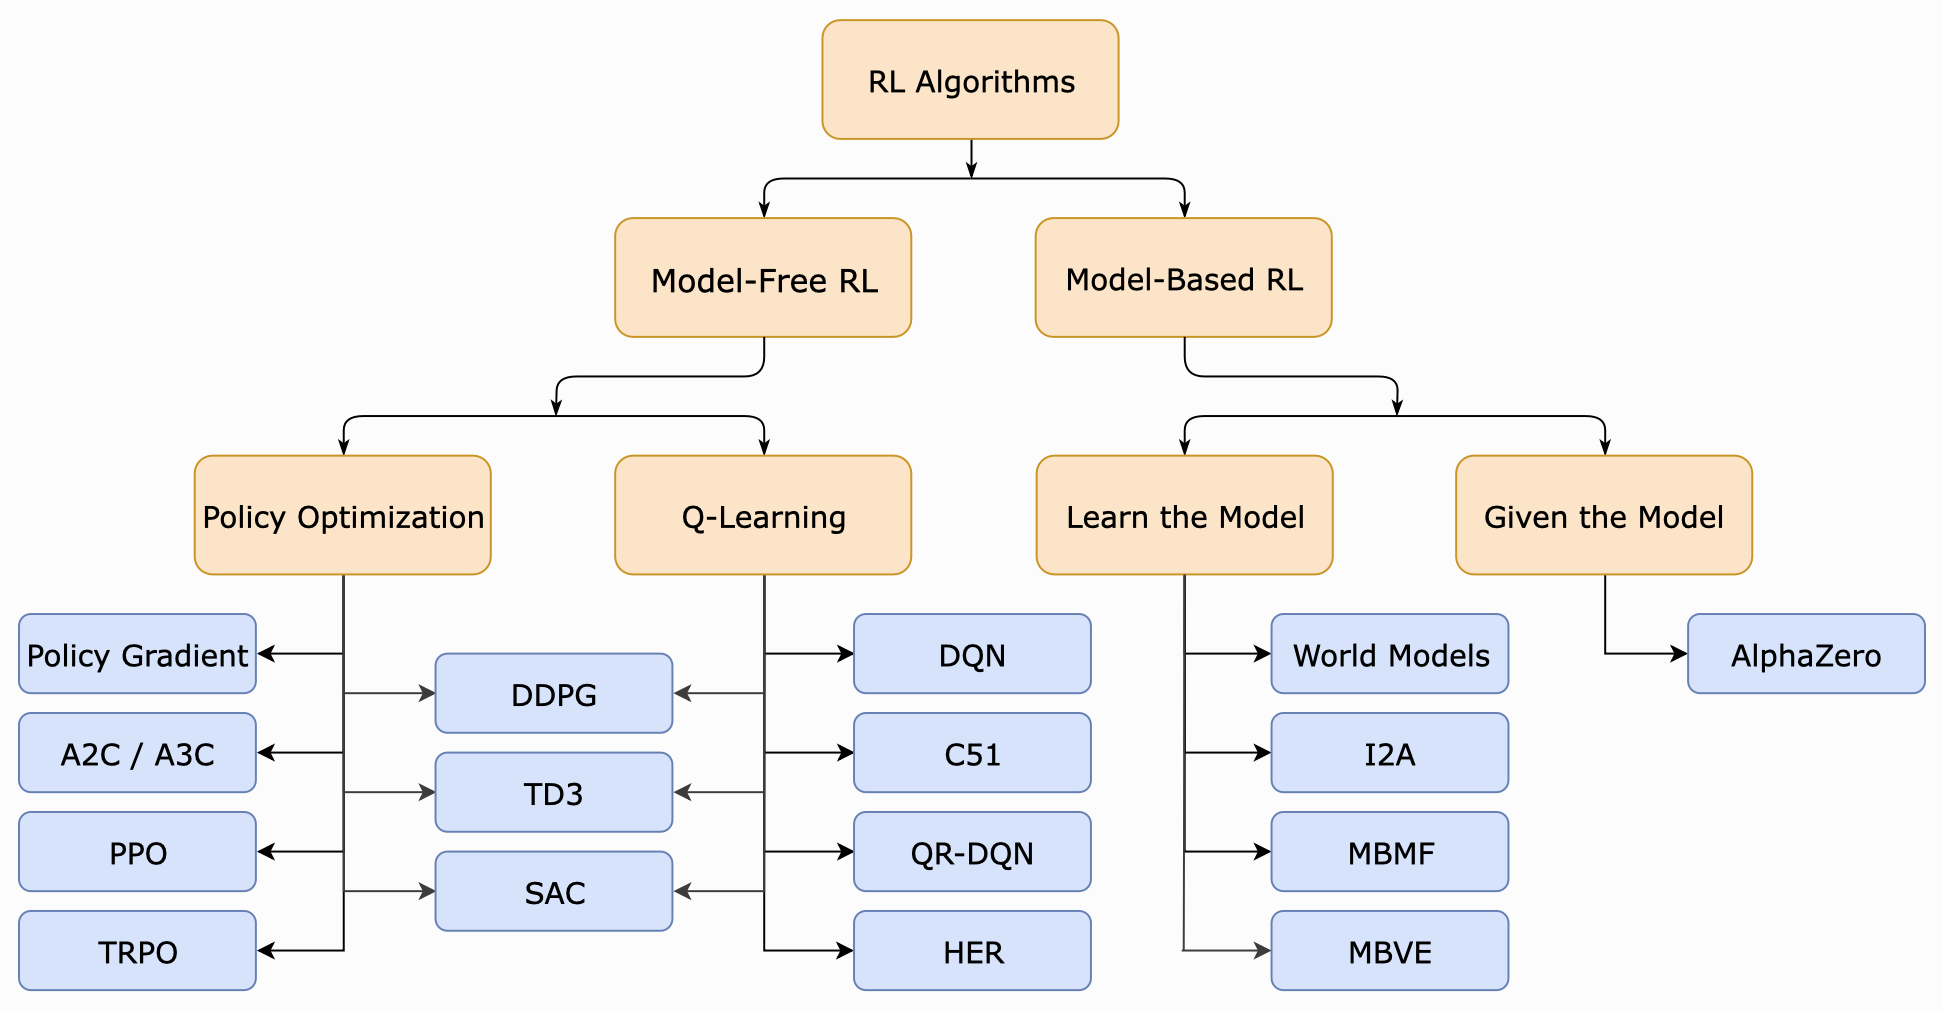
\includegraphics[width=0.8\textwidth]{figures/rl-taxonomy.png}
    \caption{Taxonomy of Reinforcement Learning Algorithms \cite{Achiam2018}}
    \label{fig:rl_taxonomy}
\end{figure}

The full potential of \acrlong{rl} algorithms is achieved when leveraging the power of \acrlong{dl} to solve dynamic stochastic control problems that have high-dimensionality in their representation of the state and action spaces. \acrshort{drl} algorithms use \acrshort{dnn}s to approximate the value functions, or use gradient ascent to find the optimal policy parameters. These thesis will focus on the following \acrshort{drl} algorithms on policy-based and actor-critic algorithms.

\subsubsection{Advantage Actor-Critic (A2C)} \label{sec:a2c}

The \acrfull{a2c} algorithm was developed by Mnih et al. (2016) in their paper on \textit{Asynchronous methods for deep reinforcement learning} \cite{Mnih2016}. The main contribution is the usage of the advantage function to address the variance issues present in policy gradient methods. The \acrshort{a2c} is the synchronous version of \acrshort{a3c}, and is preferred due to its better performance in terms of training time and cost-effectiveness \cite{Wu2017}.

The algorithm consists of a dual-network architecture, where the actor network learns a stochastic policy $\pi\left(a_t\mid s_t; \theta\right)$ and the critic network learns the value function $V\left(s_t; \theta_v\right)$. The policy and the value function are updated after every $t_max$ actions or when a terminal state is reached. The advantage function is estimated as follows: 
\begin{equation}
    A\left(s_t, a_t; \theta, \theta_v\right) = \sum_{i=0}^{k-1} \gamma^i r_{t+i} + \gamma^k V\left(s_{t+k}; \theta_v\right) - V\left(s_t; \theta_v\right)
\end{equation}
where $k$ represents the $n$-step return and is upper-bounded by the maximum number of steps $t_{max}$, and $\gamma$ is the discount factor. The algorithm's objective function is defined as:
\begin{equation}
    J\left(\theta, \theta_v\right) = \mathbb{E}_{\pi}\left[\log \pi\left(a_t\mid s_t; \theta\right) A\left(s_t, a_t; \theta, \theta_v\right)\right]
\end{equation}

The pseudo-code for the algorithm for \acrshort{a2c} is outlined in appendix \ref{alg:a2c}. 

\subsubsection{Proximal Policy Optimization (PPO)} \label{sec:ppo}

\acrfull{ppo} is a policy gradient algorithm that was introduced by Schulman et al. (2017) in their paper on \textit{Proximal Policy Optimization Algorithms} \cite{Schulman2017} with the objective of constraining policy updates. The algorithm balances sufficiently large policy updates in order to improve the policy, while avoiding excessively large changes that could hinder performance. 

\acrshort{ppo} improves the performance of \acrfull{trpo} \cite{Schulman2015} by using a clipped surrogate objective function, by ensuring that the probability ratio $r_t$ is bounded within a range of $[1 - \epsilon, 1 + \epsilon]$, where $\epsilon$ is a hyperparameter that controls the clipping range. The objective function is defined as:
\begin{equation}
    L_t^{CLIP}(\theta) = \mathbb{E}_t \left[\min\left(r_t(\theta) \hat{A}_t, \text{clip}\left(r_t(\theta), 1 - \epsilon, 1 + \epsilon\right) \hat{A}_t\right)\right]
\end{equation}
where 
\begin{equation}
    r_t(\theta) = \frac{\pi_\theta(a_t | s_t)}{\pi_{\theta_{old}}(a_t | s_t)}
\end{equation}
is the probability ratio between the current policy $\pi_\theta$ and the old policy $\pi_{\theta_{old}}$

Another improvement with respect to \acrshort{trpo} is the use of simple first-order optimisation methods as opposed to the second-order methods used in \acrshort{trpo}. Consequently, \acrshort{ppo} maintains the stability and reliability of other trust-region methods, while being easier to implement and more computationally efficient. The pseudo-code for the algorithm for \acrshort{ppo} is outlined in appendix \ref{alg:ppo}.

\subsubsection{Deep Deterministic Policy Gradient (DDPG)} \label{sec:ddpg}

\acrfull{ddpg} is an off-policy actor-critic algorithm that was introduced by Lillicrap et al. (2015) in their paper on \textit{Continuous control with deep reinforcement learning} \cite{Lillicrap2015}. The algorithm arises to solve the challenges of applying \acrlong{dqn} \cite{Mnih2013} to continuous action spaces by applying \acrfull{dpg}, which enables the efficient computation of the policy gradient without the need to integrate over the action space. 

The algorithm uses two networks: the actor network $\mu(s_t; \theta_\mu)$, which learns a deterministic policy, and the critic network $Q(s_t, a_t; \theta_Q)$, which learns the state-action value function, in conjunction with their respective target networks. The actor network is updated using \acrshort{dpg}: 
\begin{equation}
    \nabla_{\theta_\mu} J \approx \mathbb{E}_{s_t \sim \mathcal{D}} \left[\nabla_a Q(s_t, a_t; \theta_Q) \nabla_{\theta_\mu} \mu(s_t; \theta_\mu)\right]
\end{equation}
where $\mathcal{D}$ is the replay buffer that stores the agent's experiences, and the critic network is updated using the \Gls{bellmanequations}:
\begin{equation}
    \nabla_{\theta_Q} J \approx \mathbb{E}_{s_t \sim \mathcal{D}} \left[\left(r_t + \gamma Q(s_{t+1}, \mu(s_{t+1}; \theta_\mu); \theta_Q') - Q(s_t, a_t; \theta_Q)\right) \nabla_{\theta_Q} Q(s_t, a_t; \theta_Q)\right]
\end{equation}
where $\theta_Q'$ are the parameters of the target critic network. 

From \acrlong{dqn}, the algorithm incorporates a replay buffer to store the agent's experiences, which allows the agent to learn from past experiences and improve its performance over time. Moreover, \acrshort{ddpg} incorporates noise, typically Ornstein-Uhlenbeck noise \cite{Uhlenbeck1930}, to the actions taken by the actor network to encourage exploration of the action space. The pseudo-code for the algorithm for \acrshort{ddpg} is outlined in appendix \ref{alg:ddpg}.

\subsubsection{Twin Delayed Deep Deterministic Policy Gradient (TD3)} \label{sec:td3}

\acrfull{td3} is an extension of \acrshort{ddpg} introduced by Fujimoto et al. (2018) in their paper on \textit{Addressing Function Approximation Error in Actor-Critic Methods} \cite{Fujimoto2018}. The proposal addresses the hyper-parameter sensitivity and overestimation bias present in the critic network of \acrshort{ddpg}. There are three main improvements to \acrshort{ddpg}:
\begin{itemize}
    \item \textbf{Clipped Double Q-Learning}: The algorithm employs two critic networks and uses their minimum value to compute the target value for the actor network, which reduces the overestimation bias. 
    \item \textbf{Delayed Policy Updates}: The actor and critic networks updates are performed at different frequencies. The critic networks are updated every time step, whereas the actor and target networks are updated less frequently. The main benefit is that it allows the critic to improve the accuracy of the value estimates before the actor updates its policy.
    \item \textbf{Target Policy Smoothing}: The algorithm adds noise to the target action during the critic updates to smooth the value function over similar actions, resulting in a lower impact of approximation errors and more robust policies. 
\end{itemize}

The pseudo-code for the algorithm for \acrshort{td3} is outlined in appendix \ref{alg:td3}.

\subsubsection{Soft Actor-Critic (SAC)} \label{sec:sac}

\acrfull{sac}, despite being an off-policy actor-critic algorithm, represents a paradigm shift in \acrshort{rl}. The algorithm was presented by Haarnoja et al. (2018) in their paper on \textit{Soft Actor-Critic: Off-Policy Maximum Entropy Deep Reinforcement Learning with a Stochastic Actor} \cite{Haarnoja2018} and is based on the maximum entropy framework, which aims to maximise both the expected return and the entropy of the policy, encouraging the agent to succeed at the task while acting as randomly as possible. 

The algorithm uses two critic networks to estimate the state-action value function, and a stochastic actor network that learns a policy that maximises the expected return while also maximising the entropy of the policy. The critic networks are updated using the Bellman equations, and the actor network is updated using the policy gradient method. The objective function for the actor network is defined as:
\begin{equation}
    J(\theta) = \mathbb{E}_{s_t \sim \mathcal{D}} \left[\mathbb{E}_{a_t \sim \pi_\theta} \left[\alpha \log \pi_\theta(a_t | s_t) + Q(s_t, a_t; \theta_Q)\right]\right]
\end{equation}
where $\alpha$ is a temperature parameter that controls the trade-off between exploration and exploitation, and $\mathcal{D}$ is the replay buffer that stores the agent's experiences. The critic networks are updated using the Bellman equations:
\begin{equation}
    J(\theta_Q) = \mathbb{E}_{s_t \sim \mathcal{D}} \left[\left(r_t + \gamma \min_{i=1,2} Q(s_{t+1}, \mu_\theta(s_{t+1}) + \mathcal{N}(0, \sigma); \theta_{Q_i}) - Q(s_t, a_t; \theta_{Q_i})\right)^2\right]
\end{equation}
where $\mathcal{N}(0, \sigma)$ is the noise added to the action to encourage exploration, and $\theta_{Q_i}$ are the parameters of the two critic networks. The temperature parameter $\alpha$ is learned automatically by maximising the entropy of the policy, which is defined as:
\begin{equation}
    J(\alpha) = \mathbb{E}_{s_t \sim \mathcal{D}} \left[\alpha \log \pi_\theta(a_t | s_t)\right]
\end{equation}
This parameter is used to control the trade-off between the entropy and the reward terms, effectively controlling the stochasticity of the policy.

The pseudo-code for the algorithm for \acrshort{sac} is outlined in appendix \ref{alg:sac}.
